\documentclass{article}
\usepackage[utf8]{inputenc}
\usepackage{tikz}

\title{Pagerank Estimation with Deep Graph Networks}
\author{Timo Denk, Samed Güner}
\date{June 2019}

\begin{document}

\maketitle

\section{Introduction}
General description, open problems, motivation, goals of this work, contributions, structure

\section{Background}
Methods, literature, related work (perhaps as a separate subsection)
Description of GCP, K8s, infrastructure background

\subsection{Ground Truth}
\subsubsection{Open Page Rank}
\label{OpenPageRank}

\section{Method}
Our contributions, novel aspects, great detail

% Datasets Section

\section{Datasets}
In our approach we propose a supervised machine learning algorithm to estimate the page rank using deep graph networks. For this purpose we require labelled data to develop, train and validate our model. 

In general the process of gathering, augmenting and labelling of data can take an immense amount of time and slow down the development of machine learning model. Therefore we decided to iteratively develop and align our dataset to the current need of research and progress of development. For each upcoming iteration we specified the requirements for the data set. Following from this each iteration resulted in an own data set version.

The following sections will profoundly specify each dataset version as required during the development of our approach.

\subsection{Dataset Version 1}
\label{DatasetVersion1}
The dataset version 1 consists of 100000 samples in total. The ground truth for this dataset version is \textit{OpenPage Rank}, which is described in \ref{OpenPageRank}.

Every sample $k$ is a tuple consisting of three values and corresponds to one Domain $D$ from the ground truth:

\begin{center}
 $ k \in (I_D, R_D, U_D)$
\begin{itemize}
	\item[$I_D$]: The screenshot of the domain $D$ in image format PNG and in the resolution 1920x1080.
	\item[$R_D$] $\in [1, 100000]$ : The global rank of the domain $D$, according to Open PageRank (\ref{OpenPageRank}). 
	\item[$U_D$]: The URL of the domain $D$ mapped by the Open PageRank list. Example: \textit{github.com}
\end{itemize}
\end{center}

\subsection{Dataset Version 2}
\label{DatasetVersion2}
The dataset version 2 consists of 100000 samples in total and the ground truth is \textit{Open PageRank} as described in dataset version 1.

Every sample $k$ is mapped to a domain $D$ from the ground truth and represents a tuple consisting of four values:

\begin{center}
$k \in (U_D,R_D,H_D,G_D)$
\begin{itemize}
	 \item[$U_D$]: The URL of the domain $D$ mapped by the Open PageRank list.
	\item[$R_D$] $\in [1, 100000]$ : The global rank of the domain $D$ according to Open PageRank (\ref{OpenPageRank}). 
    \item[$H_D$] $\in \{true, false\}$: Indicator for whether the website uses the protocol HTTPS.
    \item[$G_D$] $= (V_D, A_D)$: The directed graph of the domain $D$ characterized by a set of vertices $V_D$ and arrows $A_D$.
\end{itemize}
\end{center}

\subsubsection{The Directed Graph}
The directed graph provides a topological view on the given website by representing all associated webpages within the same domain as vertices and connections as arrows as in figure \ref{fig:PartialDirectedGraph_timodenk.com} exemplary illustrated. During the crawling process as described in \ref{Datacrawler} vertices and arrows of the graph are created and enriched with local information about the visited webpages.

The directed graph $G_D$ is characterized by a set of vertices $V_D$ and arrows $A_D$. Each vertices $v \in V_D$ represents a webpage $p$ of the given domain $D$ and is characterized by the following tuple:

\begin{center}
	$v \in (U_p, I_p, M_p,T_p, L_p, S_p)$
\begin{itemize}
	\item[$ U_p$] : The exact URL of the webpage $p$. Example: \textit{https://github.com/help}
	\item[$I_p$] : The screenshot of webpage $p$ in image format PNG and in the resolution 1920x1080.
	\item[$M_p$] The screenshot of webpage $p$ in image format PNG and in mobile resolution TODO ZxY.
	\item[$T_p$] : The title of webpage $p$ as can be seen in the tabs bar of a common browser.
	\item[$L_p$] : The time it takes to download all data of webpage $p$ from the web server in milliseconds.
	\item[$S_p$] : Number of kilobytes downloaded in total for webpage $p$.
\end{itemize}
\end{center}

Each arrow represents a possible navigation from webpage $p$ to $q$ in the graph $G_D$. It can be understood as a hyperlink or button found on webpage $p$ (source), which leads to webpage $q$ (target) in the same domain $G_D$. 

\begin{center}
	$a \in (U_p, U_q, L_{p,q})$
	\begin{itemize}
		\item[$U_p$] : The source URL of the webpage $p$
		\item[$U_q$] : The target URL of the webpage $q$ the arrow directs to.
		\item[$L_{p,q}$] : If existent, the text that links from source to target webpage. 
	\end{itemize}
\end{center}

\begin{figure}
\centering
\usetikzlibrary{shapes.multipart}
  \tikzset{
	vertices/.style = {   
		text width=12.0em, align=center,                                           
		draw,
		rectangle split,
		rectangle split parts=6
	}
}
\scalebox{.85}{
\begin{tikzpicture}
\node[vertices]  (timodenk) at (5,4) {
	\nodepart{one} timodenk.com 
	\nodepart{two} 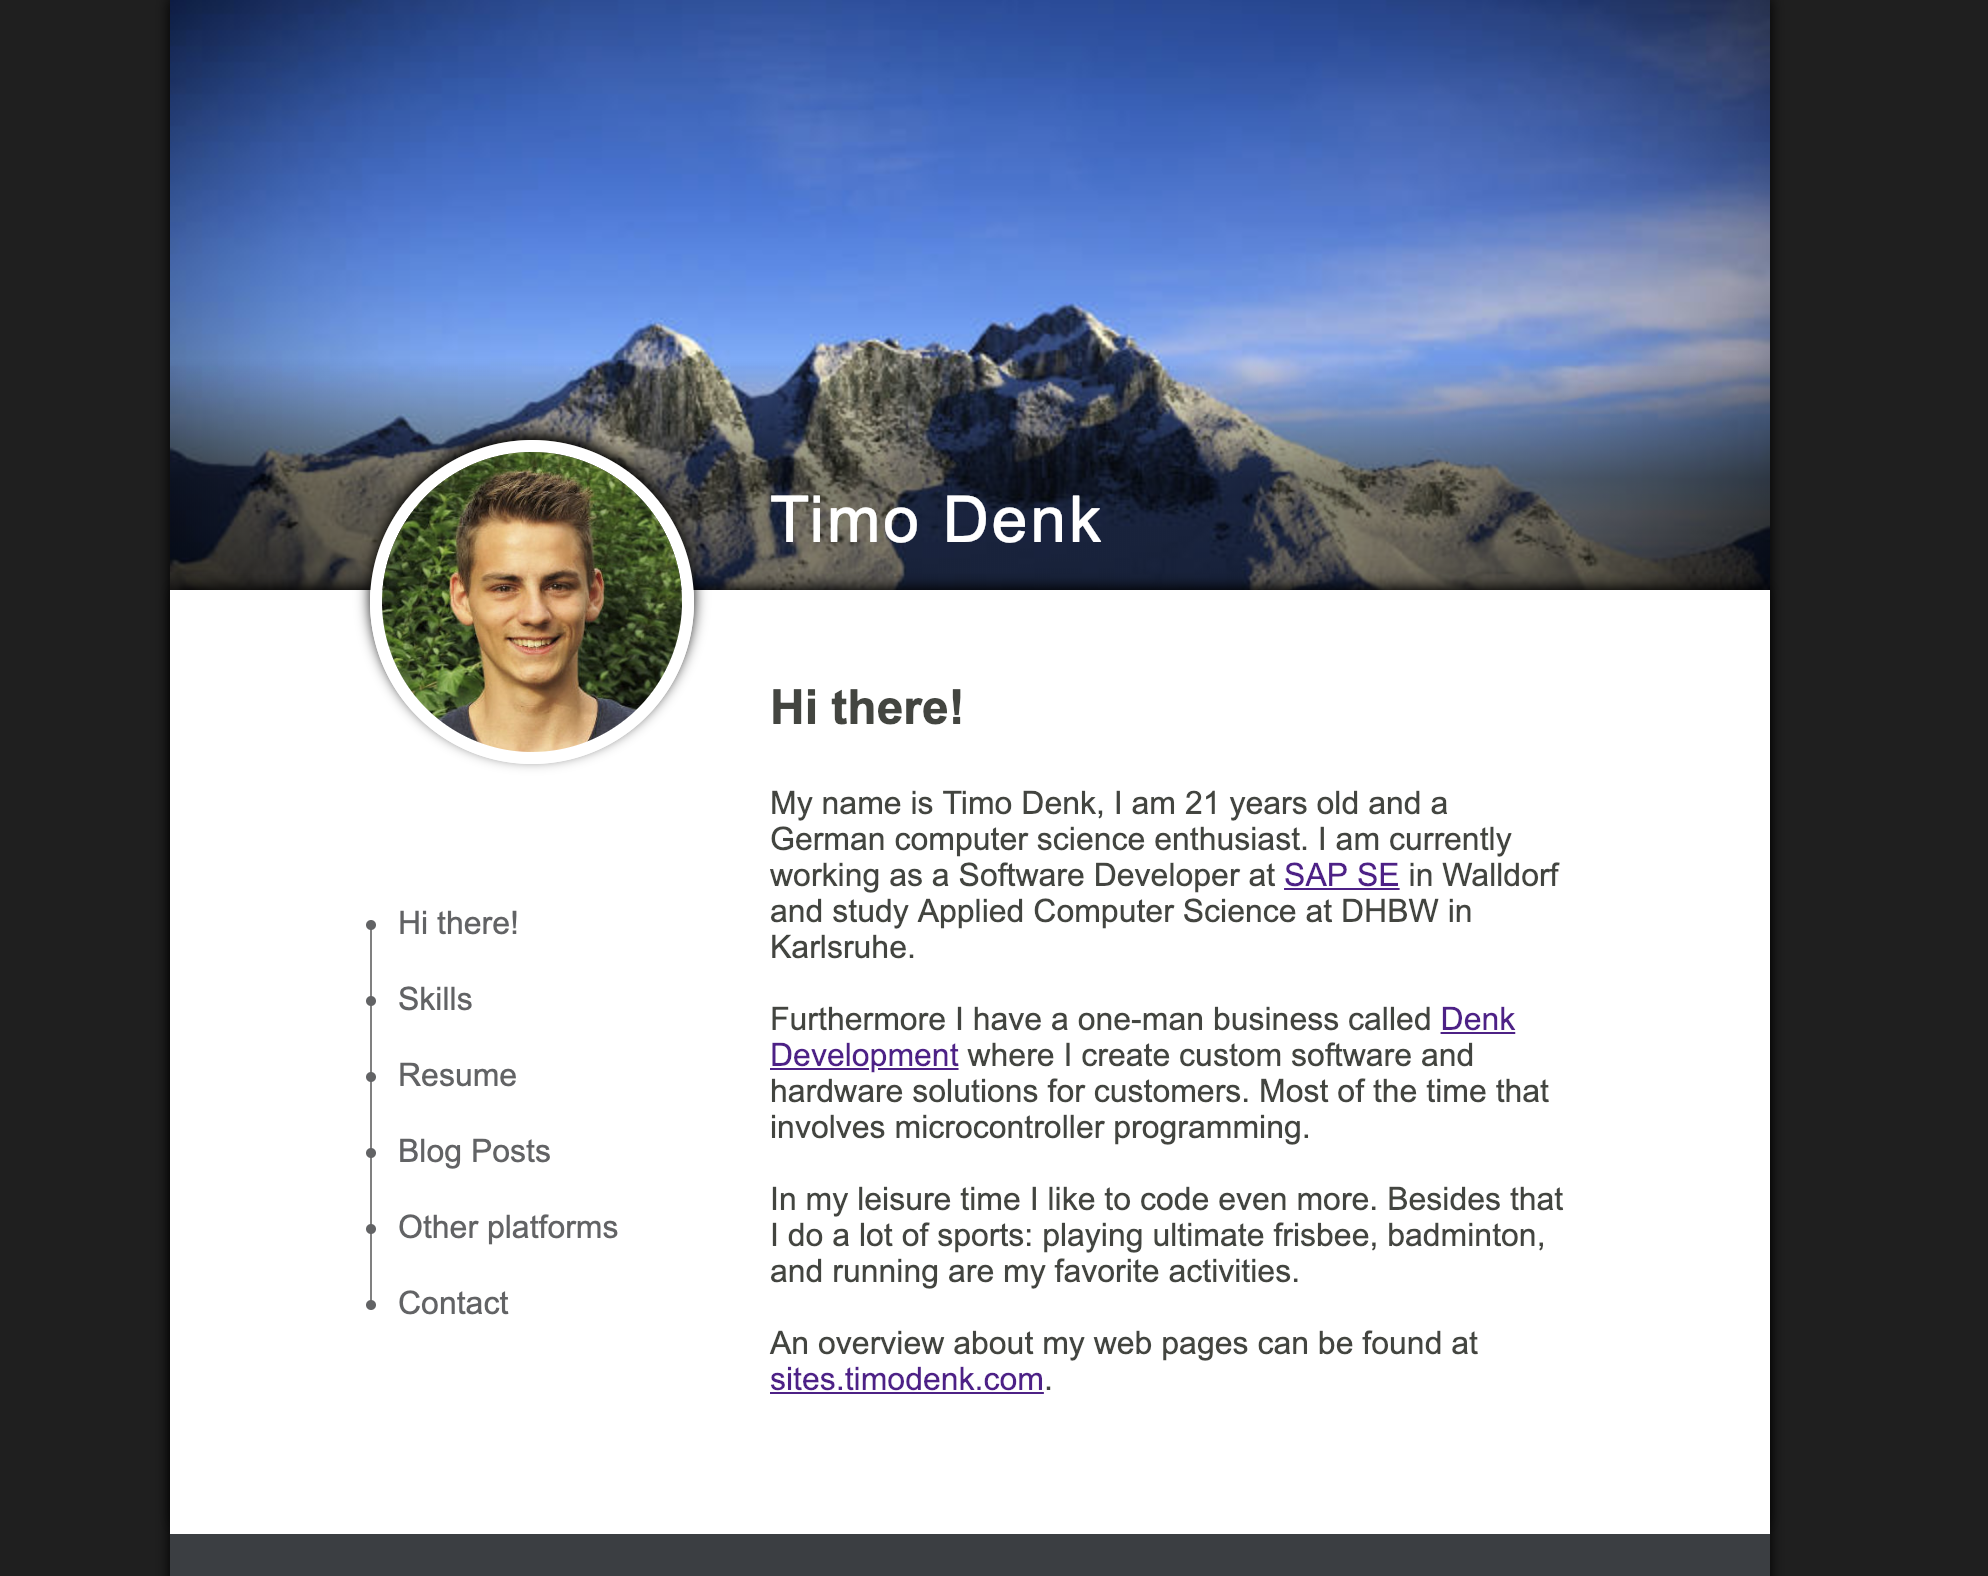
\includegraphics[width=.5\textwidth]{resources/timodenk}
	\nodepart{three} 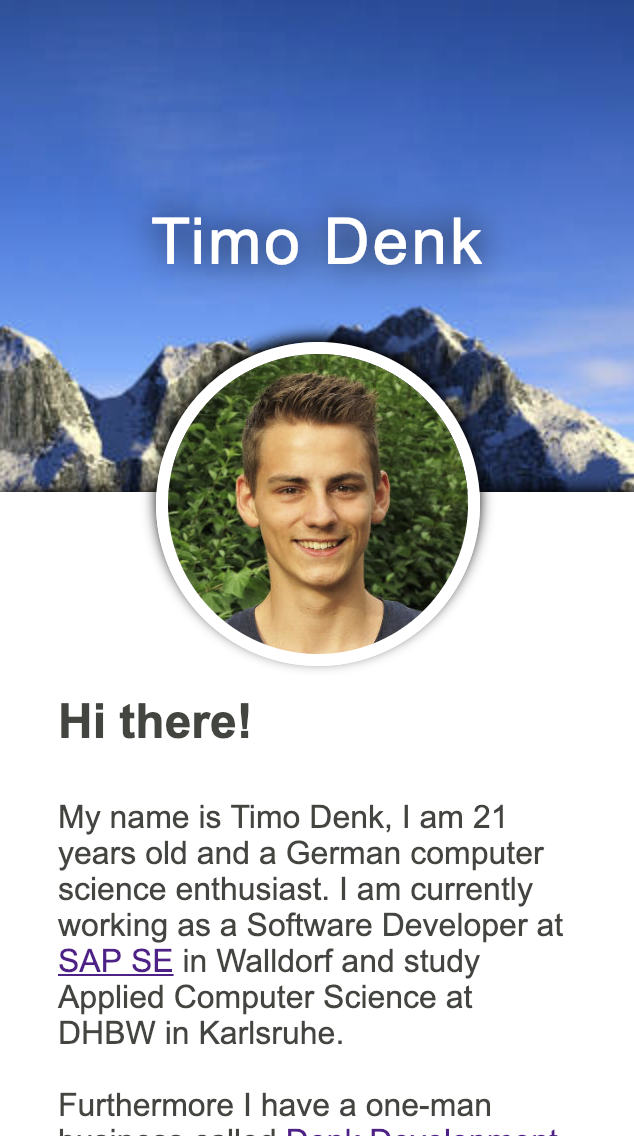
\includegraphics[width=.25\textwidth]{resources/timodenk_mobile}
	\nodepart{four} Timo Denk
	\nodepart{five} 636 ms
	\nodepart{six} 434 kb
};

\node[vertices]  (sites) at (10,2) {
\nodepart{one} sites.timodenk.com
\nodepart{two} 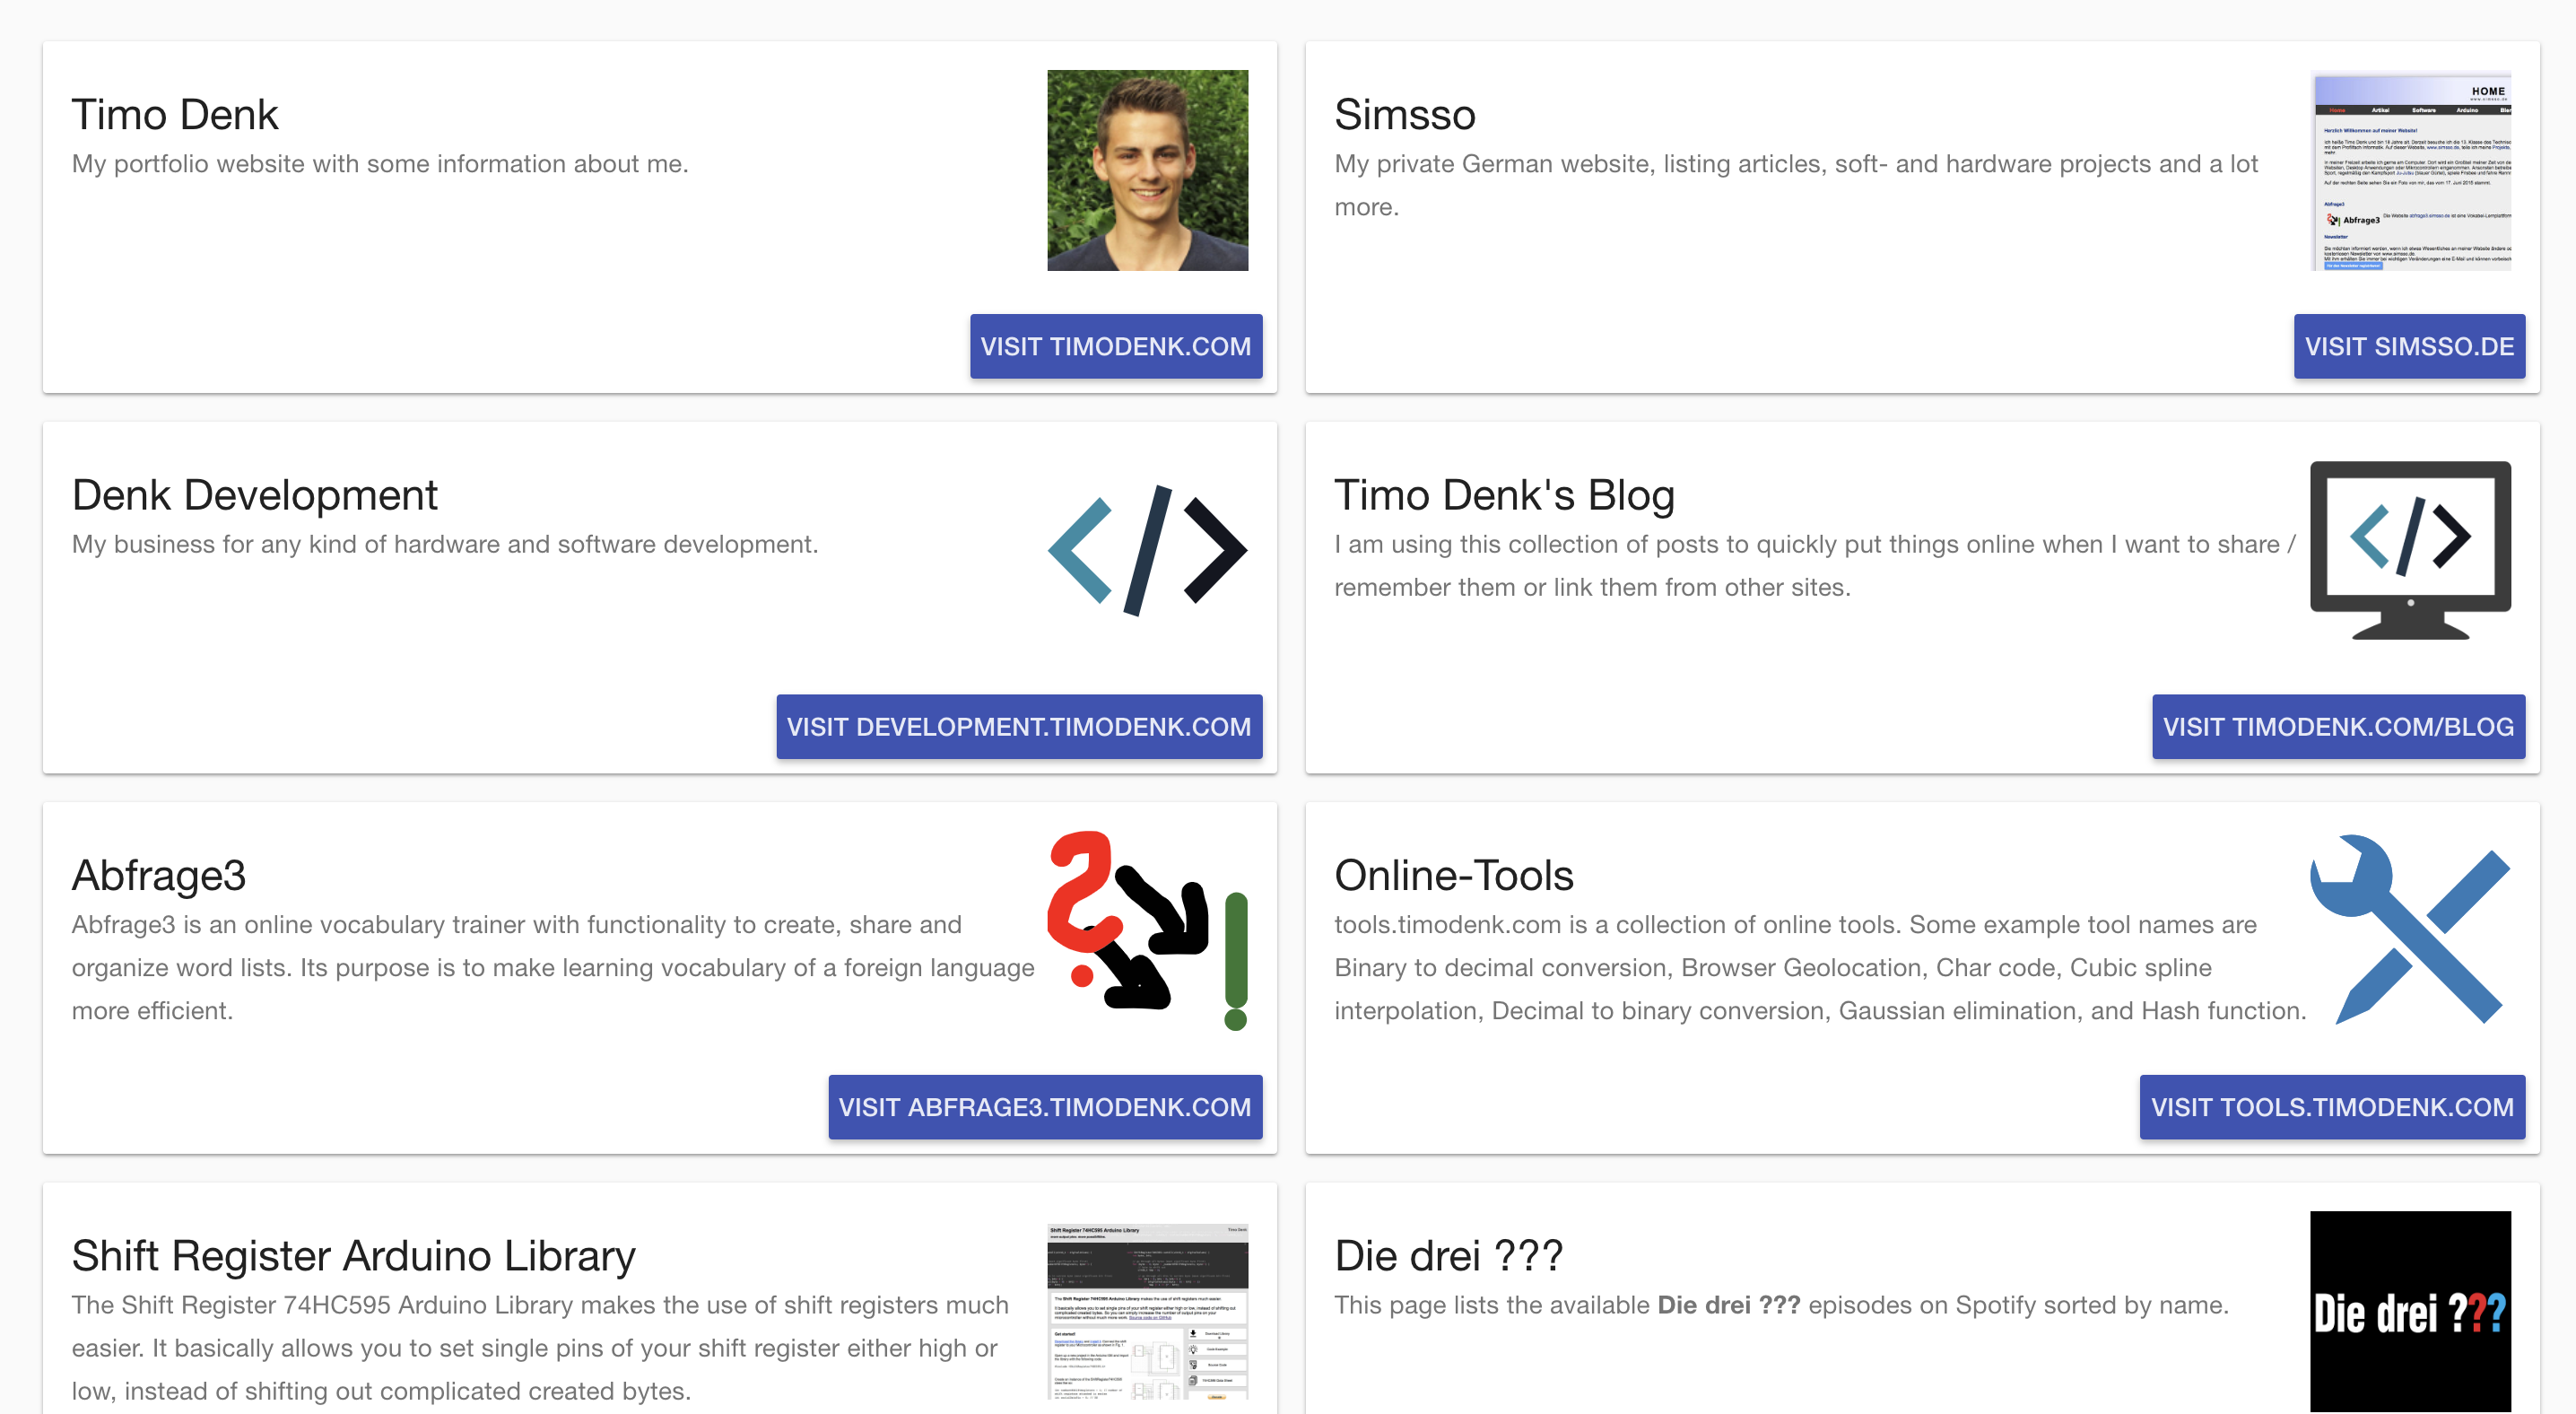
\includegraphics[width=.5\textwidth]{resources/sites_timodenk}
\nodepart{three} 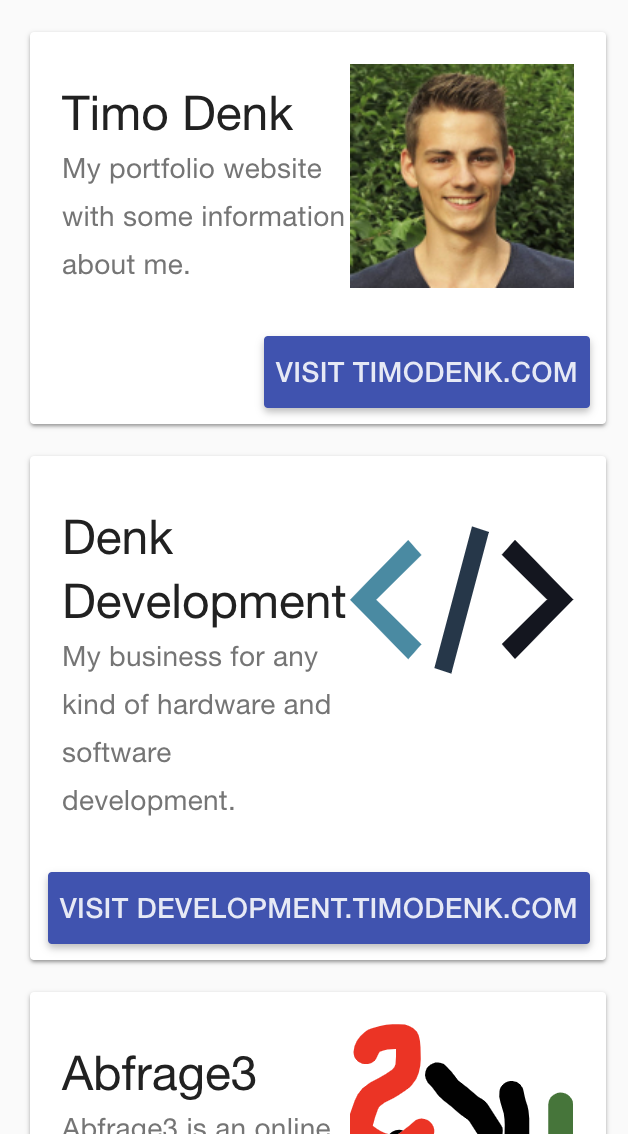
\includegraphics[width=.25\textwidth]{resources/sites_timodenk_mobile}	\nodepart{four} Timo Denk Sites Overview
\nodepart{five} 767 ms
\nodepart{six} 737 kb
};

\node[vertices]  (imprint) at (0,2) {
\nodepart{one} timodenk.com/imprint
\nodepart{two} 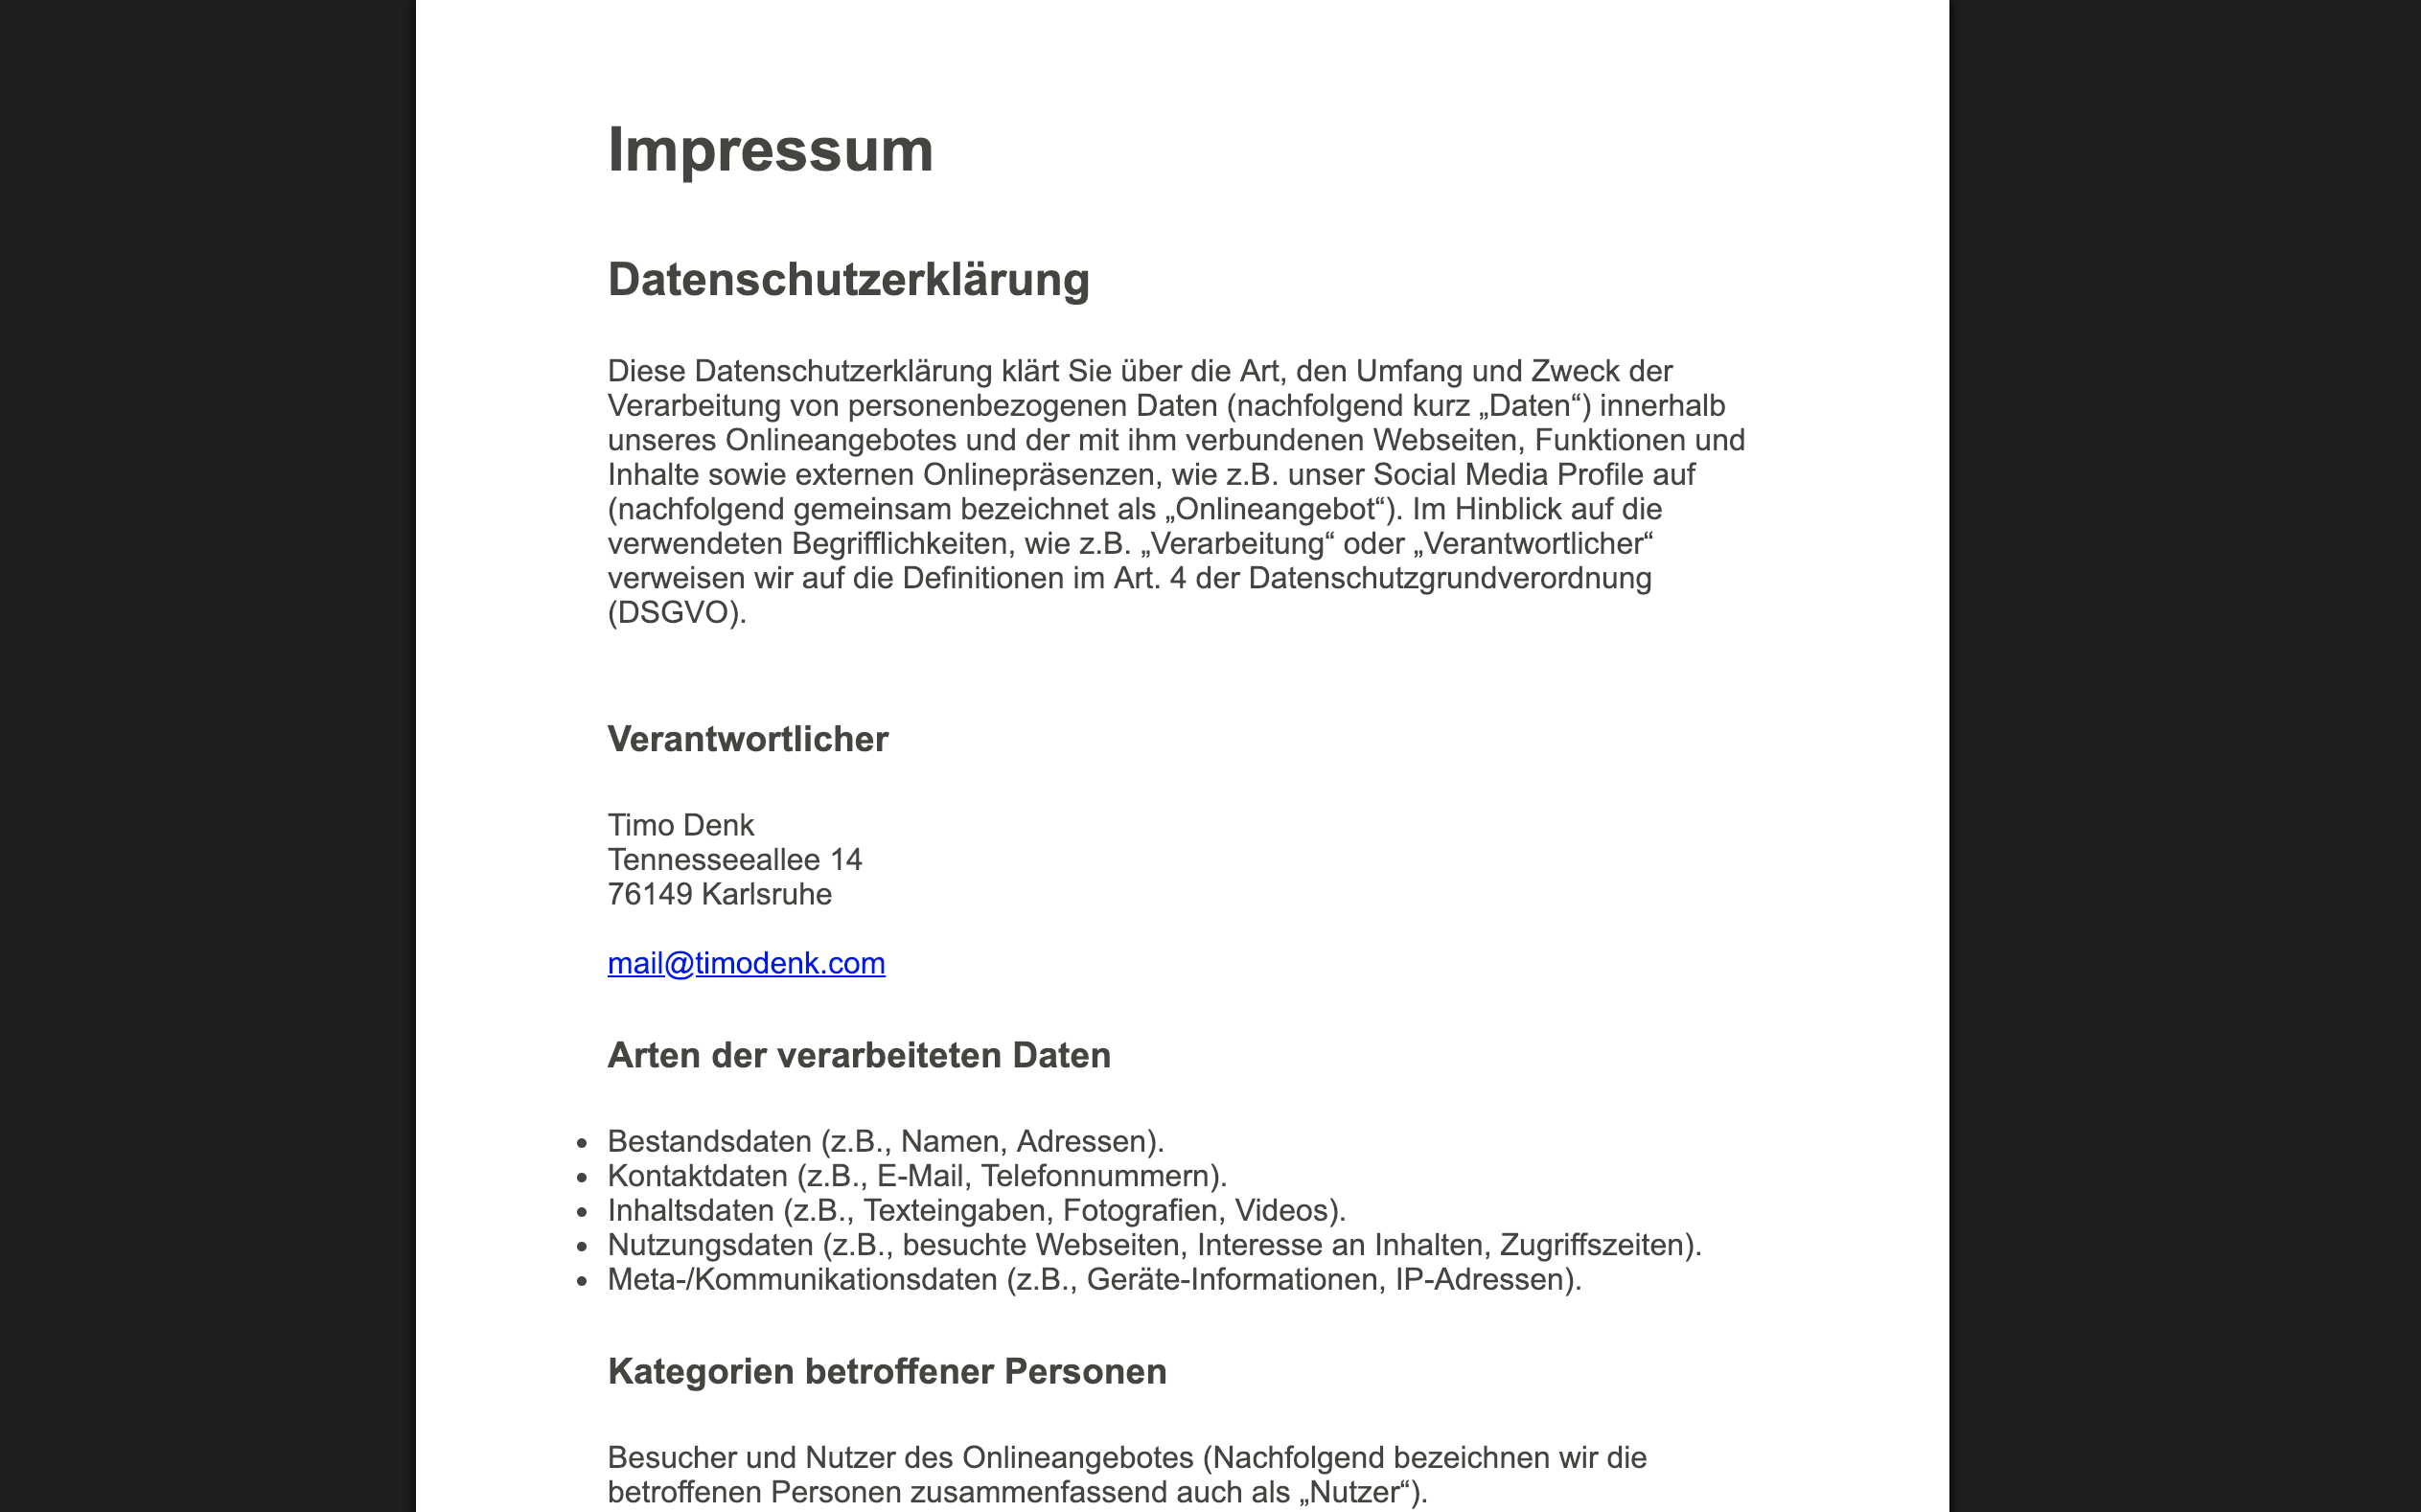
\includegraphics[width=.5\textwidth]{resources/imprint_timodenk}
\nodepart{three} 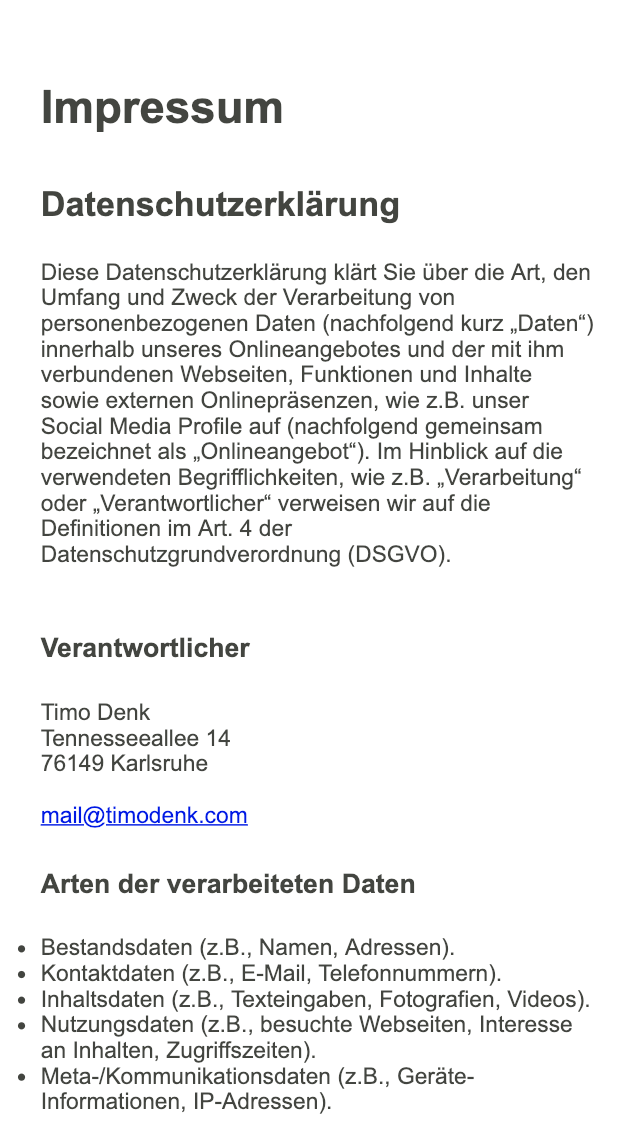
\includegraphics[width=.25\textwidth]{resources/imprint_timodenk_mobile}
\nodepart{four} Imprint - www.timodenk.com
\nodepart{five} 304 ms
\nodepart{six} 52 kb
};

\node (timodenkToImprint) at (0.5,6) {timodenk.com/imprint};
\node (timodenkToSites) at (9.5,6) {sites.timodenk.com};
\node (SitesToTimodenk) at (5.5,0.25) {timodenk.com};
\draw[-latex] (timodenk.one east) to [bend left=30] (sites.one north);
\draw[-latex] (sites.six west) to [bend left=30] (timodenk.six south);
\draw[-latex] (timodenk.one west) to [bend right=30](imprint.one north);
\end{tikzpicture}
}
\caption{Illustrates partial directed graph of domain \textit{timodenk.com} with three webpages, corresponding arrows and vertices}
\label{fig:PartialDirectedGraph_timodenk.com}
\end{figure}


\section{Implementation Details}
Technical aspects of our methods, things we have tried that might have failed, code snippets
Technical description of the dataset creation process

\section{Results}
Presentation of our results, no opinion

\section{Discussion}
Discussion of the results, assumptions about why things are the way they are

\section{Conclusion}
Summary, outlook, future work

\section{References}
Literature, papers, weblinks

\end{document}
